\documentclass[12pt, a4paper]{article}
\usepackage[english]{babel}
\usepackage[utf8x]{inputenc}
\usepackage{amsmath}
\usepackage{graphicx}
\usepackage[colorinlistoftodos]{todonotes}
\usepackage{setspace}
\usepackage{listings}






% ---------------------------------------------

\lstdefinestyle{customc}{
  belowcaptionskip=1\baselineskip,
  breaklines=true,
  frame=L,
  xleftmargin=\parindent,
  language=C,
  showstringspaces=false,
  basicstyle=\footnotesize\ttfamily,
  keywordstyle=\bfseries\color{green!40!black},
  commentstyle=\itshape\color{purple!40!black},
  identifierstyle=\color{blue},
  stringstyle=\color{orange},
}


% ----------------------------------------------



\begin{document}

\begin{titlepage}

\newcommand{\HRule}{\rule{\linewidth}{0.5mm}} % Defines a new command for the horizontal lines, change thickness here

\center % Center everything on the page
 
%----------------------------------------------------------------------------------------
%	HEADING SECTIONS
%----------------------------------------------------------------------------------------
% \linespread{1.5}
% \vspace{11cm}

{\setstretch{1.3}
	\textsc{\LARGE Hanoi University of Science and Technology}\\[0.5cm] % Name of your university/college
	\textsc{\Large School of Information and Communication Technology}\\[1.5cm] % Major heading such as course name
}



\includegraphics{logo.png}\\[1cm] % Include a department/university logo - this will require the graphicx package
%----------------------------------------------------------------------------------------
%	TITLE SECTION
%----------------------------------------------------------------------------------------

\HRule \\[0.6cm]
{\setstretch{1.75}
	{ \huge \bfseries COMPILER CONSTRUCTION REPORT}\\[0.5cm] % Title of your document
}
\HRule \\[1.5cm]

%----------------------------------------------------------------------------------------
%	AUTHOR SECTION
%----------------------------------------------------------------------------------------

% \begin{minipage}{0.45\textwidth}
% \begin{flushleft} \large
% \emph{Author:}\\
% \textsc{Hoang} Van Sam
% \end{flushleft}
% \end{minipage}
% ~
% \begin{minipage}{0.5\textwidth}
% \begin{flushright} \large
% \emph{Instructor:} \\
% Dr.\textsc{Nguyen} Thi Thu Huong
% \end{flushright}
% \end{minipage}\\[2cm]

\emph{Instructor:} Dr.Nguyen Thi Thu Huong \\
\emph{Class:} ICT 58\\
\emph{Student:} Hoang Van Sam \\[1.9cm]




% If you don't want a supervisor, uncomment the two lines below and remove the section above
%\Large \emph{Author:}\\
%John \textsc{Smith}\\[3cm] % Your name.


%----------------------------------------------------------------------------------------
%	DATE SECTION
%----------------------------------------------------------------------------------------

% {\large \today}\\[2.0cm] % Date, change the \today to a set date if you want to be precise
{\large Hanoi, December 27, 2016}\\
%----------------------------------------------------------------------------------------
%	LOGO SECTION
%----------------------------------------------------------------------------------------

 
%----------------------------------------------------------------------------------------

\vfill % Fill the rest of the page with whitespace

\end{titlepage}

%----------------------------------------------------------------------------------------
% table of contents
\tableofcontents
\clearpage
%----------------------------------------------------------------------------------------



% \begin{abstract}
% Your abstract.
% \end{abstract}
%----------------------------------------------------------------------------------------
\section{An Overview of compiler}
In this course, we learn how to build a simple compiler for KPL language
\subsection*{What's Compiler and What Compiler Does ?}
A computer program (or set of programs) that transforms source code written in a high level language into the target language, often having a binary form known as object code. \\
Simple Compiler has 4 main part as figure below
\begin{center}
	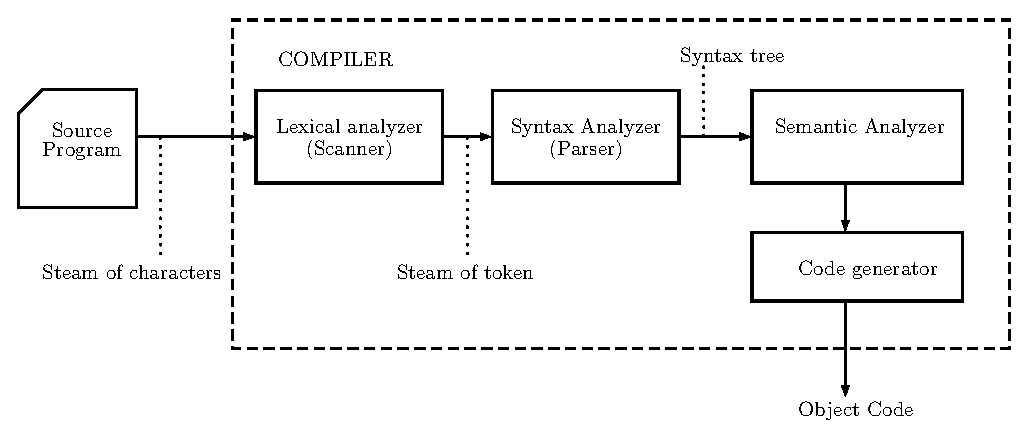
\includegraphics[width=14cm]{compiler_diagram}
\end{center}
%----------------------------------------------------------------------------------------
\section{Lexical Analyzer - Scanner}
Lexical Analyzer (Scanner) Converts the stream of input characters into a stream of tokens that becomes the input to the following phase\\

\begin{center}
	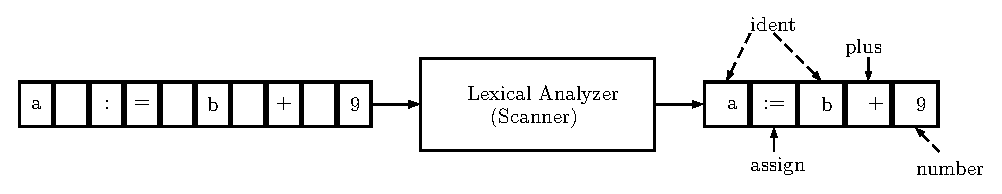
\includegraphics[width=15cm]{lex}
\end{center}
\clearpage
\subsection*{Problems need to be solve in Scanner}
\begin{itemize}
	\item Skip meaningless characters (blank, tab, new line character, comment)
	\item Recognize illegal character and return error message
	\item Recognize different types of token
	\item Pass recognized tokens to the parser 
\end{itemize}

In order to recognize different types of token we define a stucture and use Deterministic Finite Automaton (DFA)\\

\lstinputlisting[caption=Token Structure, language=C]{tokenStruct.h}

\clearpage

One of difficult problems in this Scanner is skip comment, in order to solve it, we use Deterministic Finite Automaton (DFA)\\
% code 



\lstinputlisting[caption=Skip Comment Function, language=C]{skipComment.c}


\clearpage

\section{Syntax Analyzer - Parser}
Syntax Analyzer is 2nd pharse of a compiler. Tasks of a Parser is check the syntactic structure of a given program and Invoke semantic analysis and code generation\\
KPL is LL(1) language, we use top-down parser without backtrack\\
\subsection*{Design Top-down parser}
\begin{itemize}
	\item \textbf{lookAhead} token
	\item Parsing terminals
	\item Parsing non-terminals
		\begin{itemize}
			\item Constructing a parsing table
			\begin{itemize}
				\item Computing \textbf{FIRST()} and \textbf{FOLLOW()}	
			\end{itemize}		
		\end{itemize}
\end{itemize}


\lstinputlisting[caption=Data Structure use in parser, language=C]{parserStruct.h}

Scan function use for change currentToken to lookAhead andget new lookAhead token\\
\lstinputlisting[caption=Scan function, language=C]{scanParser.c}

Eat function use for check currentToken if currentToken is expected token type then invoke scan functio else it will has an error\\
\lstinputlisting[caption=Eat function, language=C]{eatParser.c}

\section{Semantic Analyzer}
Semantic Analyzer is 3nd pharse of a compiler. It check components of a program fit together meaningfully\\
\subsection*{Task of Semantic analyzer}
\begin{itemize}
	\item Create Symbol Table
	\item Scope Checking
	\item Type Checking
\end{itemize}


\lstinputlisting[caption=Data Structure of Symbol Table, language=C]{symDS.h}

% \lstinputlisting[caption=Data Structure of Object, language=C]{objSt.h}

In order to check type or check kind of Object, we need to find it first.

\lstinputlisting[caption=Function for Lookup (Find) Object, language=C]{lookupSen.c}

\lstinputlisting[caption=List function for check Declare, language=C]{checkDec.h}

\lstinputlisting[caption=List function for check Type, language=C]{checkType.h}

\end{document}